\section{Ciepły start}\label{chapter:results_warm_start}

Pierwszym kryterium badanym w testach wydajnościowych był czas działania funkcji podczas ciepłych startów.
Oznacza to sytuację, gdy funkcja była wywołana w momencie, gdy aktywna była jedna z instancji funkcji.
Powoduje to, że nie jest wymagana inicjalizacja usługi, a kod rozpoczyna działanie bezpośrednio po wywołaniu.
Średni czas wykonania w zależności od metody i rozmiaru pamięci został przedstawiony na Rysunku \ref{fig:avg_warm_start}.
Dokładne wartości oraz różnica względem funkcji bazowej (Java JVM) zostały zaprezentowane w Tabeli \ref{table:warm_start_comparison}.

\begin{figure}[h]
    \centering
    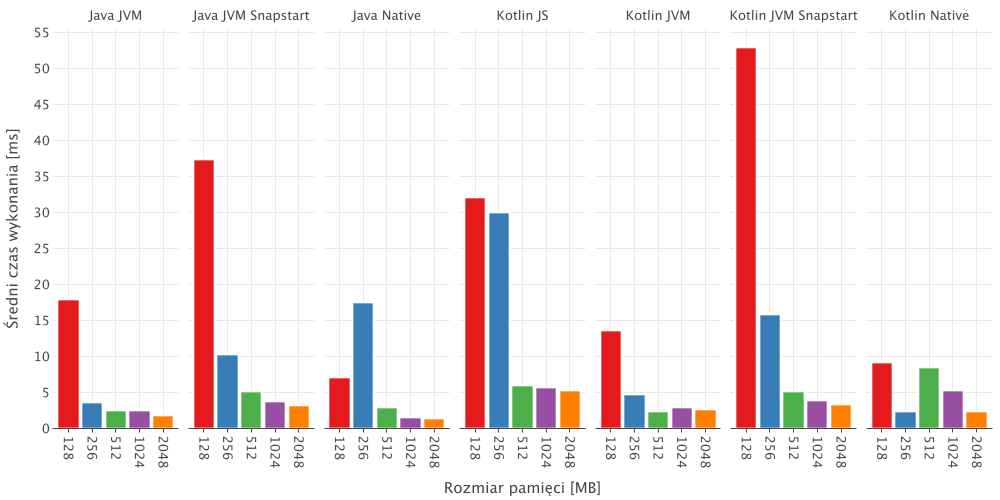
\includegraphics[width=0.95\textwidth]{charts/results/avg-warm-start.png}
    \caption{Średni czas wykonywania funkcji (ciepły start) z użyciem wybranych metod w zależności od rozmiaru pamięci [źródło: opracowanie własne]}
    \label{fig:avg_warm_start}
\end{figure}

Dla każdego z badanych rodzajów funkcji widoczne jest znaczne zróżnicowanie czasu wykonania w zależności od rozmiaru pamięci.
Sama skuteczność metod w poprawie wydajności różni się także ze względu na pamięć funkcji.
Pierwsza metoda, czyli usługa SnapStart, nie przyniosła poprawy czasu wykonania w żadnej z badanych wielkości pamięci.
Zastosowanie obrazów natywnych GraalVM pozwala na zmniejszenie czasu w niektórych rozmiarach pamięci: 128 MB, 1024 MB oraz 2048 MB.
Podobnie zachowuje się funkcja napisana w Kotlinie, działające w ramach JVM: tutaj poprawa jest widoczna dla pamięci 128 MB i 512 MB.

Funkcja działające w oparciu o kod JavaScript, stworzony poprzez translację Kotlin/JS, niesie negatywny wpływ na czas wykonania.
Metoda ta nie przyniosła poprawy w żadnym z badanych rozmiarów pamięci, przy czym w małych rozmiarach (128 MB, 256 MB) wpłynęła znacząco negatywnie na wydajność.
Dodatkowo, nie widać znacznej poprawy efektywności wraz z wzrostem rozmiaru pamięci z 512 MB do 2048 MB. 
Ciekawa zależność widoczna jest w przypadku funkcji Kotlin/Native, która wskazuje wykazuje poprawę czasu działania dla małych wielkości pamięci (128 MB i 256 MB).
Szczególna poprawa widoczna jest dla rozmiaru 256 MB, gdzie metoda ta osiągnęła niższe czasy wykonania niż funkcja Java JVM dla większych wielkości pamięci (512-2048 MB).

\begin{table}[h]
    \caption{Porównanie średnich czasów działania funkcji podczas ciepłego startu względem funkcji bazowej [źródło: opracowanie własne]}
    \centering
    \begin{tabular}{|>{\raggedright\arraybackslash}p{3.5cm}| >{\raggedright\arraybackslash}p{1.8cm}| >{\raggedright\arraybackslash}p{1.8cm}| >{\raggedright\arraybackslash}p{1.8cm}| >{\raggedright\arraybackslash}p{1.8cm}| >{\raggedright\arraybackslash}p{1.8cm}|}
    \hline
    \multirow{2}{*}{\makecell[l]{\textbf{Rodzaj funkcji} \\ \scriptsize{\textit{Czas [ms] (\% różnicy)}}}} & \multicolumn{5}{c|}{\textbf{Rozmiar pamięci [MB]}} \\
    \cline{2-6} 
    & \textbf{128} & \textbf{256} & \textbf{512} & \textbf{1024} & \textbf{2048} \\
    \hline
    Java JVM & 17.88 & 3.65 & 2.55 & 2.47 & 1.81 \\
    \hline
    Java JVM + SnapStart & 37.36 \mbox{(109\%)} & 10.3 \mbox{(182\%)} & 5.14 \mbox{(102\%)} & 3.74 \mbox{(51\%)} & 3.25 \mbox{(80\%)} \\
    \hline
    Java GraalVM & 7.08 \mbox{(-60\%)} & 17.47 \mbox{(379\%)} & 2.87 \mbox{(13\%)} & 1.47 \mbox{(-40\%)} & 1.39 \mbox{(-23\%)} \\
    \hline
    Kotlin JVM & 13.55 \mbox{(-24\%)} & 4.7 \mbox{(29\%)} & 2.41 \mbox{(-5\%)} & 2.88 \mbox{(17\%)} & 2.62 \mbox{(45\%)} \\
    \hline
    Kotlin JVM + SnapStart & 52.91 \mbox{(196\%)} & 15.87 \mbox{(335\%)} & 5.12 \mbox{(101\%)} & 3.88 \mbox{(57\%)} & 3.4 \mbox{(88\%)} \\
    \hline
    Kotlin/JS & 32.15 \mbox{(80\%)} & 29.97 \mbox{(721\%)} & 5.93 \mbox{(133\%)} & 5.65 \mbox{(129\%)} & 5.25 \mbox{(190\%)} \\
    \hline
    Kotlin/Native & 9.19 \mbox{(-49\%)} & 2.37 \mbox{(-35\%)} & 8.44 \mbox{(231\%)} & 5.3 \mbox{(115\%)} & 2.35 \mbox{(30\%)} \\
    \hline
    \end{tabular}
    \label{table:warm_start_comparison}
\end{table}

Na Rysunkach \ref{fig:warm_start_256} oraz \ref{fig:warm_start_1024} przedstawiono wykresy pudełkowe z czasami wykonania funkcji dla rozmiarów pamięci 256 MB i 1024 MB.
Funkcje oparte wyłącznie o maszynę wirtualną wykazały najmniej zróżnicowane wyniki.
Aktywacja funkcji SnapStart znacząco obniżyła stabilność czasów odpowiedzi, podobnie jak Kotlin/JS.
Warte zwrócenia uwagi są jednak funkcje natywne. 
Obrazy GraalVM wykazują jednolite wyniki, oprócz pamięci 256 MB, gdzie czas wykonania znacząco różnił się w poszczególnych wywołaniach.
Podobna zależność występuje dla funkcji Kotlin/Native, które osiągają niestabilne wyniki dla rozmiarów pamięci 512 MB oraz 1024 MB.

% --- Row 1: 256 MB and 1024 MB charts ---
\begin{figure}[h]
    \centering % Center the minipages on the line
    \begin{minipage}[t]{0.48\textwidth} % [t] for top alignment
        \centering % Center content within this minipage
        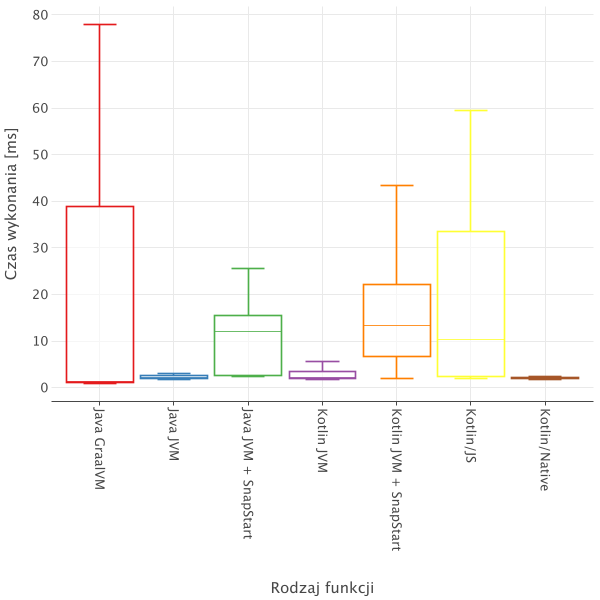
\includegraphics[width=\linewidth]{charts/results/warm-start-boxplot-256.png}
        \captionof{figure}{Czas wykonania funkcji (ciepły start, 256 MB) [źródło: opracowanie własne]}
        \label{fig:warm_start_256} % Unique label for this figure
    \end{minipage}% <--- % is important
    \hfill % Space between minipages
    \begin{minipage}[t]{0.48\textwidth}
        \centering
        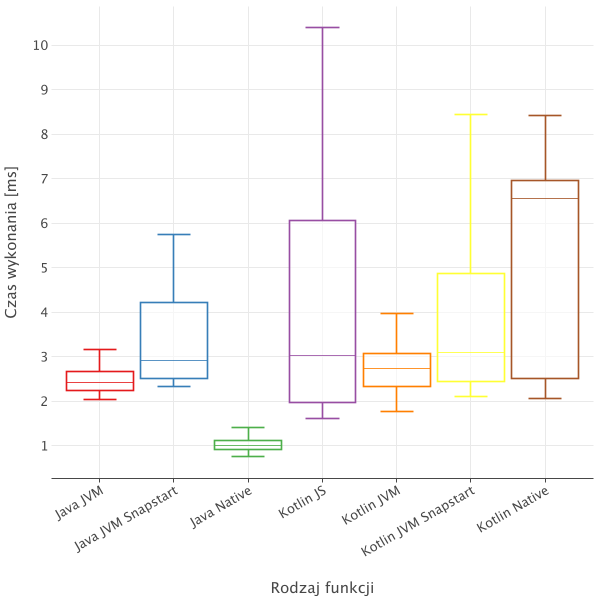
\includegraphics[width=\linewidth]{charts/results/warm-start-boxplot-1024.png}
        \captionof{figure}{Czas wykonania funkcji (ciepły start, 1024 MB) [źródło: opracowanie własne]}
        \label{fig:warm_start_1024} % Unique label
    \end{minipage}
    % No overall \caption for this outer figure environment, as it's just for layout.
\end{figure}
